% pdflatex new.tex %
\documentclass{article}

\usepackage{graphicx}

\title{Deep Learning Topic Based Sentiment Analysis}
\author{Berti Stefano}
\date{\today}

\begin{document}
    \thispagestyle{plain}
    % Titles %
    \begin{center}
        \Large
        \textbf{Deep Learning Topic Based Sentiment Analysis}

        \vspace{0.4cm}
        \large Human Language Technologies
        \\2019 / 2020

        \vspace{0.4cm}
        \textbf{Berti Stefano}

        \vspace{0.9cm}
        \textbf{Abstract}
    \end{center}
    % Abstract %
    The aim of this project is to apply the model
    \\\centerline{https://github.com/cbaziotis/datastories-semeval2017-task4}
    To the Aspect Category Polarity task of the Absita competition
    \\\centerline{http://sag.art.uniroma2.it/absita}
    To show the strength of the proposed model.
    I will also try to apply the same model to the Aspect Category Detection task and I will try two different word
    vectors strategies: the Italian Word2Vec (https://mlunicampania.gitlab.io/italian-word2vec/) and the Italian BERT
    AlBERTo (https://github.com/ marcopoli/AlBERTo-it)


    \section{Task, dataset and metrics}\label{sec:s1}
        The Absita competition is divided into 2 tasks:
        \begin{itemize}
            \item \textbf{ACD}: Aspect Category Detection, to understand which topic is dealt inside the review
            \item \textbf{ACP}: Aspect Category Polarity, given a review and a topic, understand if the topic is dealt in a positive, negative, neutral or mixed way
        \end{itemize}
        Obviously the second task is dependent from the first one, but we will see it as a independent tasks
        because otherwise, the results of the second task couldn't be better than the result of the first task.
        I transformed the given dataset in order to obtain a tsv file of the form
        \\\centerline{id, topic, y, review}
        where
        \begin{itemize}
            \item \textbf{id} is the id of the review
            \item \textbf{topic} is one element in $['cleanliness', 'amenities', 'value', 'wifi', 'location', 'staff', 'other']$
            \item \textbf{y} in ACP task, this refers to the sentiment of the review towards that topic and it is an element in $['positive', 'negative', 'neutral', 'mixed']$, in ACD task this refers if the topic is dealt in the review or not and it is an element in $['positive', 'negative']$
            \item \textbf{review} is the raw review
        \end{itemize}
        \begin{table}[h!]
            \begin{center}
                \caption{element for class}
                \label{tab:table1}
                \begin{tabular}{l|c|c|c|r}
                    \textbf{data} & \textbf{positive} & \textbf{neutral} & \textbf{mixed} & \textbf{negative}\\
                    \hline
                        train & 4942 & 0 & 173 & 3797\\
                        test & 2080 & 0 & 64 & 1757\\
                \end{tabular}
            \end{center}
        \end{table}
        Since I didn't have a single element for neutral review neither in train set nor test set, I decided to remove it from the possible classes.
        The metrics used in this competition were $micro-precision$, $micro-recall$ and $f1-score$.

    \section{Description of the models}\label{sec:s3}
        The model chosen is the one who wins the $Semeval2017$, which tasks were very similar to this one.
        It is a deep-learning model with context-aware attention:
        \begin{itemize}
            \item The inputs are word indices to be embedded in the EmbeddingLayer for the Word2Vec version or sentences already embedded for the AlBERTo version (with topics and sentiments, of course)
            \item It feeds each embedding in a LSTM. It does the same with the topic using the same weights in order to try to get meaningful representation.
            \item It concatenates each word representation with the topic representation
            \item It uses a context-aware attention mechanism, which tries to understand which part of the reviews contribute more to understand better sentiment/references towards the topic
            \item It feeds those representations in a dense layer with a single sigmoid neuron for task ACD and 3 softmax neurons for task ACP
        \end{itemize}
        \begin{figure}
            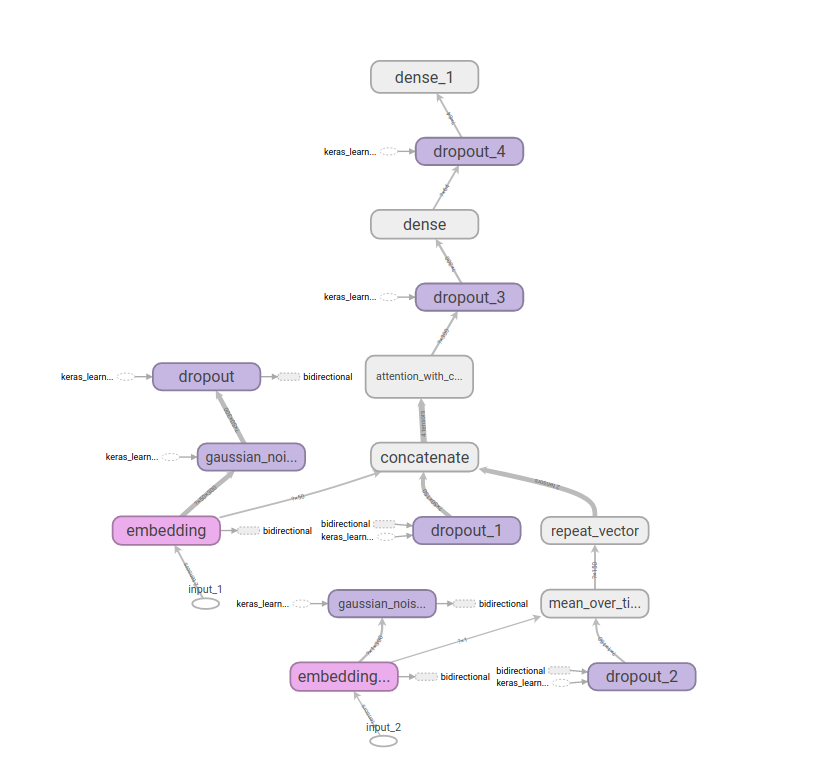
\includegraphics[width=\linewidth]{w2v_model.png}
            \caption{The model that uses Word2Vec}
            \label{fig:w2v_model}
        \end{figure}
            \begin{figure}
            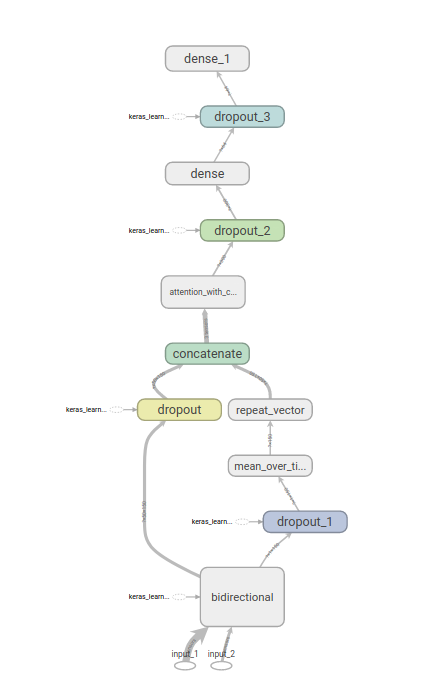
\includegraphics[width=\linewidth]{alberto_model.png}
            \caption{The model that uses AlBERTo}
            \label{fig:alberto_model}
        \end{figure}

    \section{Experiments}\label{sec:s4}
        \subsection{ACP}\label{subsec:s1}
            \begin{figure}
                \includegraphics[width=\linewidth]{../experiments/acp/plots.png}
                \caption{Training plot for acp task}
                \label{fig:train-acp}
            \end{figure}
            Initially I only considered the positive and negative classes because of the very few mixed samples, by assigning to
            mixed reviews a random sentiment, and, although this gives nice results, I moved from a one sigmoid output neuron for
            positive and negative class, to 3 softmax output neurons for positive, negative and mixed class.
            I used class weights, which help dealing with imbalanced datasets by weighting more the misclassified prediction of a class
            with a limited number of example.
            In my case the class weights used were 1.26 for negative, 1.0 for positive and 8.14 for mixed.
            \subsubsection{Word2Vec}
            Embeddings are given in a txt file, but after the first loading, they are formatted as dictionary and saved in a pickle file
            to speed up following loading.
            Initially I made some experiments using a word embedding whose dimension was 128 (http://www.italianlp.it/resources/italian-word-embeddings/), but this lead to a slow and limited training, that couldn't overtake the accuracy score of 0.55, which was very bad.
            So I moved to a more informative embeddings which size is 300, and although the big dimension of 2.4GB and the poor quality of most of the entries, it gives good results.
            I didn't do a lot of preprocessing of the reviews, since the embedding size is big (667564 words once removed the non-ascii ones) and it could cover the 85\% of the words, but looking better at the words that were indexed as $<unk>$, a lot of them were words with a capital letter.
            So by setting all chars lowercase, without losing much information because no proper name was present in the dataset, and just by removing all \textbf{l'}, the coverage of ward embeddings increased to 95\%.
            This can be increased more correcting typo using edit distance for example, but I did not investigating further since this improved coverage improved my metrics by more or less 0.04, that was what I needed.
            \subsubsection{AlBERTo}
            I used Huggingface Transformers to download AlBERTo model and tokenizer, then I decided to generate an "AlBERTed" version of the dataset,
            in this way I don't need to calculate the embeddings during the training because I have already computed them,
            and this result in a faster training at the cost to spend time and space to generate and save it.
            The tokenizer managed to index all the words.
            The dimension of these embeddings is 768, which is much larger than the Word2Vec ones

        \subsection{ACD}\label{subsec:s2}
            \begin{figure}
                \includegraphics[width=\linewidth]{../experiments/acd/plots.png}
                \caption{Training plot for acd task}
                \label{fig:train-acd}
            \end{figure}
            Even if this model was not designed for topic-detection analysis, I experimented a way to understand its potential and limit.
            So I proceed modifying the dataset in such a way to only detect if a topic is dealt in a review, and not in which way it is dealt.
            The idea is that the context-aware attention should learn which words refers to a specific topic.
            So I tried various probability to add a negative sample (see ACD dataset description) since I obtain both class weights around 1.0, hoping that a balanced dataset could give better results.
            I also had to create negative samples for the ACD train and test set, since obviously I only had positive samples.
            In order to do so, for each review $r$ and for each absent topic $t$ I added the sample $("negative", t, r)$ with a certain probability, that I set to value 0.2.

            \subsubsection{Word2Vec}

            \subsubsection{AlBERTo}


    \section{Results}\label{sec:s5}
        I had the official gold test set during training, but I didn't use it for model selection since that would have been incorrect.
        So the model selection is based on the highest validation recall.
        I used the official evaluation\_absita script for calculate the scores.
        \begin{itemize}
            \item \textbf{ACD results}: the obvious and only way to predict the presence of topic in a sentence, is to try each topic for each sentence and collect the positive results only.
                %ACD RESULTS
                \begin{table}[h!]
                    \begin{center}
                        \caption{independent results for ACP task}
                        \label{tab:table2}
                        \begin{tabular}{l|c|c|c|r}
                            \textbf{model} & \textbf{Micro-Precision} & \textbf{Micro-Recall} & \textbf{Micro-F1-score}\\
                            \hline
                                absita best model & 0.8397 & 0.7837 & 0.8108\\
                                my model & 0.6832 & 0.8204 & 0.7455\\
                        \end{tabular}
                    \end{center}
                \end{table}
            \item \textbf{ACP results}: this results can be calculated in two ways: using the output of the previous task as input, or create a new input based on the right presence of topics in sentences.
                In the first way, the results obviously is dependent from the result of the first task, in particular the score cannot be higher than what we obtain from the ACD task.
                % ACP DEPENDENT DESULTS
                \begin{table}[h!]
                    \begin{center}
                        \caption{DEPENDENT results for ACP task}
                        \label{tab:table3}
                        \begin{tabular}{l|c|c|r}
                            \textbf{model} & \textbf{Micro-Precision} & \textbf{Micro-Recall} & \textbf{Micro-F1-score}\\
                            \hline
                                absita best model & 0.8264 & 0.7161 & 0.7673\\
                                my model & 0.3675 & 0.4366 & 0.3991\\
                        \end{tabular}
                    \end{center}
                \end{table}
                In the second way, we test the model with correct topic, leading to a better analysis of this task
                % ACP INDEPENDENT RESULTS
                \begin{table}[h!]
                    \begin{center}
                        \caption{INDEPENDENT results for ACP task}
                        \label{tab:table4}
                        \begin{tabular}{l|c|c|r}
                            \textbf{model} & \textbf{Micro-Precision} & \textbf{Micro-Recall} & \textbf{Micro-F1-score}\\
                            \hline
                                absita best model & 0.8264 & 0.7161 & 0.7673\\
                                my model & 0.9277 & 0.9162 & 0.9219\\
                        \end{tabular}
                    \end{center}
                \end{table}
        \end{itemize}
        Obviously the second way is not possible if we don't have the gold test data, so for completeness i considered both cases.



    \section{Conclusion}\label{sec:s6}
        Deep-Learning approaches with context-attention has difficulty to understand the topics dealt in reviews.
        This could be due to a small dataset, which contains few element for each topic class.
        Simpler statistical approaches like LinearSVC gives us better results, arund 90\% for each class, thanks to lemmatization which reduces the vocabulary and has fewer elements to analyze.
        Nevertheless, the model is very good at understanding the sentiment towards a certain topic, and it can also understand if the sentiment towards a topic are mixed, and in different topics have different sentiments in the same review.

    \section{Other plots}\label{sec:s7}
            \begin{figure}
                \includegraphics[width=\linewidth]{../experiments/acp/no_onehot.png}
                \caption{Training plot for acp task with only two classes [positive, negative]}
                \label{fig:train-acd-no-onehot}
            \end{figure}
                \begin{figure}
                \includegraphics[width=\linewidth]{../experiments/acp/without_preprocessing.png}
                \caption{Training plot for acp task with 3 output neurons, but embeddings coverage of 85\% instead of 95\%}
                \label{fig:train-acd-no-preprocessing}
            \end{figure}
\end{document}